\documentclass[conference]{IEEEtran}
\usepackage[utf8]{inputenc}
\usepackage[T1]{fontenc}
\usepackage[spanish,es-tabla]{babel}
\usepackage{amsmath,amssymb}
\usepackage{graphicx}
\usepackage{booktabs}
\usepackage[hidelinks]{hyperref}

\graphicspath{{figs/}}

\begin{document}

\title{Emotion Is All You Need\\
{\large\normalfont Representaciones auto-supervisadas y ensembles para el
reconocimiento de emociones en el habla}}

\author{
\IEEEauthorblockN{Bautista Garcia}
\IEEEauthorblockA{Universidad de San Andrés\\garciab@udesa.edu.ar}
\and
\IEEEauthorblockN{Tomas Gonzalez}
\IEEEauthorblockA{Universidad de San Andrés\\tgonzalez@udesa.edu.ar}
}

\maketitle

\begin{abstract}
El reconocimiento de emociones en el habla (SER) busca detectar el estado
afectivo de una persona a partir de su voz, con aplicaciones que van de la
atención al cliente a la salud. En este trabajo armamos un sistema de SER
sobre RAVDESS comparando dos familias de representaciones (las features
expertas eGeMAPS y los embeddings auto-supervisados de wav2vec~2.0, WavLM y
HuBERT) y una escalera de modelos de complejidad creciente, desde Random
Forest y regresión logística hasta redes densas, recurrentes y
\emph{fine-tuning} end-to-end. Con validación cruzada estricta por hablante
(GroupKFold-5), un ensemble ponderado de clasificadores lineales sobre
varios backbones SSL más una red densa entrenada con aumentación de
pseudo-hablantes llega a $0{,}890$ de accuracy ($0{,}888$ de macro-F1),
partiendo de un baseline de $0{,}465$. La normalización por hablante (CMVN)
resultó la mejora individual más grande ($+7$ puntos), y los modelos de
mayor capacidad no superaron al enfoque lineal con los datos disponibles.
Evaluado sin reentrenar sobre EMODB (en alemán), el sistema conserva
$0{,}767$ de accuracy sobre las seis clases compartidas, y de nuevo es CMVN
lo que explica la mayor parte de la recuperación frente al cambio de
dominio.
\end{abstract}

\begin{IEEEkeywords}
reconocimiento de emociones en el habla, aprendizaje auto-supervisado,
ensembles, normalización por hablante, cambio de dominio
\end{IEEEkeywords}

\section{Introducción}

Detectar la emoción de una persona a partir de su voz tiene aplicaciones bien
concretas. En un centro de atención al cliente, por ejemplo, serviría para
monitorear cómo evoluciona el ánimo de los agentes a lo largo de sus llamadas
y detectar desgaste a tiempo, sin agregar nada a la infraestructura que ya
existe, porque las llamadas ya se graban. El desafío técnico es que la señal
de voz mezcla qué se dice, quién lo dice y cómo se dice. La emoción vive en
el tercer componente, pero los dos primeros, sobre todo la identidad del
hablante, dominan la señal acústica. Un sistema entrenado sin cuidado aprende
a reconocer voces en lugar de emociones, y falla justo en el escenario de uso
real, frente a hablantes que nunca vio.

La entrada de nuestro algoritmo es una señal de audio de voz (mono, a
16~kHz, de duración variable). A partir de ella extraemos una representación
de dimensión fija y usamos clasificadores supervisados para predecir una de
ocho emociones (neutral, calma, felicidad, tristeza, enojo, miedo, disgusto y
sorpresa). Encaramos el trabajo con dos preguntas. Primero, ¿qué
representación captura mejor la emoción, las features acústicas expertas o
las aprendidas por modelos auto-supervisados (SSL)? Segundo, ¿cuánta
capacidad de modelo aguanta un dataset de $\sim$1400 ejemplos? Como
extensión, evaluamos el sistema final sin reentrenarlo sobre un corpus en
otro idioma (EMODB, en alemán) para medir el efecto del cambio de dominio.

\section{Conjunto de datos y características}

\subsection{RAVDESS}

Trabajamos con RAVDESS~\cite{ravdess}, un corpus de 24 actores profesionales
(12 mujeres y 12 hombres) que dicen dos frases léxicamente idénticas con
acento norteamericano neutro. El canal de habla tiene 1440 audios (8
emociones $\times$ 2 frases $\times$ 2 repeticiones $\times$ 2 intensidades
$\times$ 24 actores, con la excepción de la clase neutral, que solo existe
en intensidad normal y por eso tiene la mitad de ejemplares). El corpus trae
además un canal cantado (1012 audios) que usamos solo en la exploración
inicial. Todos los resultados que reportamos son sobre el canal de habla. El
desbalance de neutral motiva usar macro-F1 como métrica complementaria y
pesos por clase al entrenar.

\subsection{Variables espurias y diseño de splits}
\label{sec:splits}

El análisis exploratorio mostró que la variación entre hablantes (y entre
géneros) en las features prosódicas es comparable o mayor que la variación
entre emociones. La identidad es un \emph{confound} directo para la tarea.
Como cada actor aporta 60 audios, un split aleatorio por muestra filtraría
voces del test al entrenamiento y sobreestimaría el rendimiento. Por eso
evaluamos con GroupKFold de 5 particiones agrupando por actor, así ningún
hablante aparece a la vez en entrenamiento y evaluación.

Hay un punto que queremos dejar claro. No apartamos un conjunto de test
propio de RAVDESS, porque con 24 hablantes reservar actores para un test
separado nos dejaba muy pocos para entrenar. Todas las métricas que
reportamos son entonces de \emph{validación}, calculadas sobre las
predicciones out-of-fold de la validación cruzada. La evaluación sobre
EMODB, que el modelo no ve en ningún momento del desarrollo, es nuestro
único test realmente externo. La intensidad y el texto, balanceados por
diseño en RAVDESS, no necesitaron control extra.

\subsection{Representaciones}

Exploramos las dos familias requeridas. \textbf{eGeMAPS}~\cite{egemaps} son
88 funcionales acústicos por audio (estadísticos de F0, energía, formantes y
espectro) extraídos con openSMILE~\cite{opensmile}, el conjunto experto
estándar en SER. Los \textbf{embeddings SSL} son las representaciones
internas de wav2vec~2.0 base~\cite{wav2vec2} (95M de parámetros, 12 capas
transformer de dimensión 768), WavLM-large~\cite{wavlm} y
HuBERT-large~\cite{hubert} (ambos de 317M, con 24 capas de dimensión 1024),
pre-entrenados sobre miles de horas de habla sin etiquetas. Siguiendo a
Pepino et~al.~\cite{pepino}, tratamos la capa de la que se extrae el
embedding como un hiperparámetro a investigar en vez de quedarnos con la
última. Como preprocesamiento, todo audio se convierte a mono 16~kHz. Para
EMODB aplicamos exactamente el mismo pipeline, sin ninguna adaptación.

\subsection{EMODB para evaluación cross-corpus}

EMODB~\cite{emodb} tiene 535 audios de 10 actores en alemán con 7 emociones.
Seis coinciden con RAVDESS (neutral, felicidad, tristeza, enojo, miedo y
disgusto). Descartamos \emph{aburrimiento}, que no tiene equivalente, y
evaluamos sobre los 454 audios restantes sin reentrenar ni recalibrar el
modelo.

\section{Metodología}

\subsection{De la señal al vector de features}

Un forward por el modelo SSL produce estados ocultos
$\mathbf{h}_t^{(\ell)} \in \mathbb{R}^H$ para cada capa $\ell$ y frame $t$
(unos 50 frames por segundo). La representación de un audio en la capa
$\ell$ es el promedio temporal (\emph{mean pooling})
\begin{equation}
\mathbf{x}^{(\ell)} = \frac{1}{T} \sum_{t=1}^{T} \mathbf{h}_t^{(\ell)},
\end{equation}
y la representación multi-capa concatena las tres mejores capas del barrido,
$\mathbf{x} = [\,\mathbf{x}^{(\ell_1)};\mathbf{x}^{(\ell_2)};\mathbf{x}^{(\ell_3)}\,]$.

\subsection{Normalización por hablante (CMVN)}

Para sacarle a las features la identidad del hablante aplicamos
\emph{cepstral mean and variance normalization} por hablante. Si
$\boldsymbol{\mu}_s$ y $\boldsymbol{\sigma}_s$ son la media y el desvío de
las features del hablante $s$,
\begin{equation}
\tilde{\mathbf{x}} = (\mathbf{x} - \boldsymbol{\mu}_s) \oslash \boldsymbol{\sigma}_s ,
\end{equation}
con $\oslash$ la división elemento a elemento. Cada audio queda representado
como su desviación respecto del punto neutro de su propio hablante, que es
justo donde vive la emoción. Las estadísticas se calculan por hablante
dentro de cada conjunto, sin cruzar información entre folds.

\subsection{Modelos}

Probamos una escalera de modelos de complejidad creciente. Los
hiperparámetros salieron de la misma validación cruzada.

El \textbf{Random Forest} (el baseline requerido) usa de 300 a 400 árboles
con pesos de clase balanceados.

Para la \textbf{regresión logística}, como acá $d \gg n$ (hasta 3072
features para 1440 audios), usamos regularización fuerte con $C{=}0{,}01$
($C{=}0{,}1$ en la comparación inicial, de dimensión menor), estandarización
previa y pesos de clase balanceados.

El \textbf{MLP} tiene dos capas ocultas (512 y 256) con ReLU, batch-norm de
entrada y dropout de 0,3, y se entrena con Adam ($\eta{=}10^{-3}$, weight
decay $10^{-4}$), batch de 64 y \emph{early stopping} con paciencia 10 sobre
una validación interna estratificada del 15\% del fold de entrenamiento.

El \textbf{CRNN} busca aprovechar la dinámica temporal que el mean pooling
descarta, trabajando sobre los frames sin promediar. Tiene una Conv1D (256
canales, kernel 5), después una BiGRU (128) y al final \emph{attention
pooling}, donde el peso de cada frame se aprende como
$\alpha_t = \mathrm{softmax}_t(\mathbf{w}^\top \mathbf{o}_t)$ y el contexto
es $\mathbf{c} = \sum_t \alpha_t \mathbf{o}_t$. Cumple el requisito de
combinar capas convolucionales, recurrentes y densas.

El \textbf{fine-tuning end-to-end} ajusta el backbone SSL completo con una
cabeza de clasificación, con lr de $2\cdot10^{-5}$ y warmup del 10\% (lo
estándar para transformers pre-entrenados), el encoder convolucional
congelado, batch de 4 a 8 y early stopping.

\subsection{Aumentación de pseudo-hablantes}

Con 24 hablantes nomás, generamos variantes de cada audio que suenan como
otra persona, usando perturbación de velocidad (factores 0,9 y 1,1, que
también corren el pitch) y ruido gaussiano (SNR 20~dB). Los embeddings de
las variantes heredan la etiqueta del original y se suman únicamente al
entrenamiento, y solo si su hablante de origen pertenece al fold de train.
Si no, la misma voz (deformada) aparecería de los dos lados del split.

\subsection{Ensemble}

El modelo final combina $K$ clasificadores por votación blanda ponderada
\begin{equation}
P(y \mid a) = \frac{1}{\sum_k w_k} \sum_{k=1}^{K} w_k \, P_k(y \mid a).
\end{equation}
Los cuatro votantes son regresiones logísticas sobre WavLM-large (top-3
capas, $w{=}2$), HuBERT-large ($w{=}2$) y wav2vec2-base ($w{=}1$), más el
MLP con aumentación ($w{=}1$), cuya entrada es la concatenación de los
embeddings de WavLM-large y wav2vec2-base. Todos los
votantes trabajan sobre features con CMVN. Los pesos los elegimos por
validación cruzada entre variantes discretas.

\subsection{Protocolo de evaluación}

La métrica principal es accuracy y la complementaria macro-F1,
$\mathrm{F1}_{\text{macro}} = \frac{1}{C}\sum_{c} \mathrm{F1}_c$, que
promedia sin ponderar por soporte y por eso castiga ignorar a la clase
minoritaria (neutral). Las dos se calculan sobre las predicciones
out-of-fold del GroupKFold-5 por actor. Como dijimos en la
Sección~\ref{sec:splits}, son métricas de validación y no hay un test set
separado de RAVDESS. Para EMODB el modelo final se entrena sobre todo
RAVDESS speech y se evalúa sin reentrenamiento.

\section{Experimentos, resultados y discusión}

\subsection{Features expertas vs.\ aprendidas}

La Tabla~\ref{tab:base} compara los dos modelos base sobre las tres
representaciones iniciales. Se ven dos cosas. Primero, los embeddings SSL
superan por mucho a eGeMAPS con los dos clasificadores. Segundo, la
regresión logística, con la regularización adecuada, le gana al Random
Forest en el espacio de alta dimensión. Combinar eGeMAPS con wav2vec aporta
poco ya desde esta etapa, primera señal de una redundancia que después se
confirma.

\begin{table}[t]
\caption{Modelos base $\times$ representación (speech, GroupKFold-5).}
\label{tab:base}
\centering
\begin{tabular}{llcc}
\toprule
Modelo & Representación & Accuracy & Macro-F1 \\
\midrule
Random Forest & eGeMAPS (88) & 0,465 & 0,449 \\
Random Forest & wav2vec capa 8 (768) & 0,588 & 0,576 \\
Random Forest & combinado (856) & 0,597 & 0,582 \\
LogReg & eGeMAPS (88) & 0,518 & 0,511 \\
LogReg & wav2vec capa 8 (768) & 0,721 & 0,715 \\
LogReg & combinado (856) & \textbf{0,727} & \textbf{0,721} \\
\bottomrule
\end{tabular}
\end{table}

\subsection{¿Qué capa del modelo SSL?}

La Figura~\ref{fig:sweep} muestra el barrido por capa para los dos
backbones. El patrón se repite en ambos. El rendimiento sube hasta las capas
intermedias y cae hacia las últimas, que están especializadas en el objetivo
de pre-entrenamiento (predecir unidades enmascaradas) y descartan
información prosódica. Nos quedamos con las tres mejores capas de cada
backbone (8-6-7 en wav2vec2-base, 13-11-10 en WavLM-large y 13-14-12 en
HuBERT-large) y las concatenamos.

\begin{figure}[t]
\centering
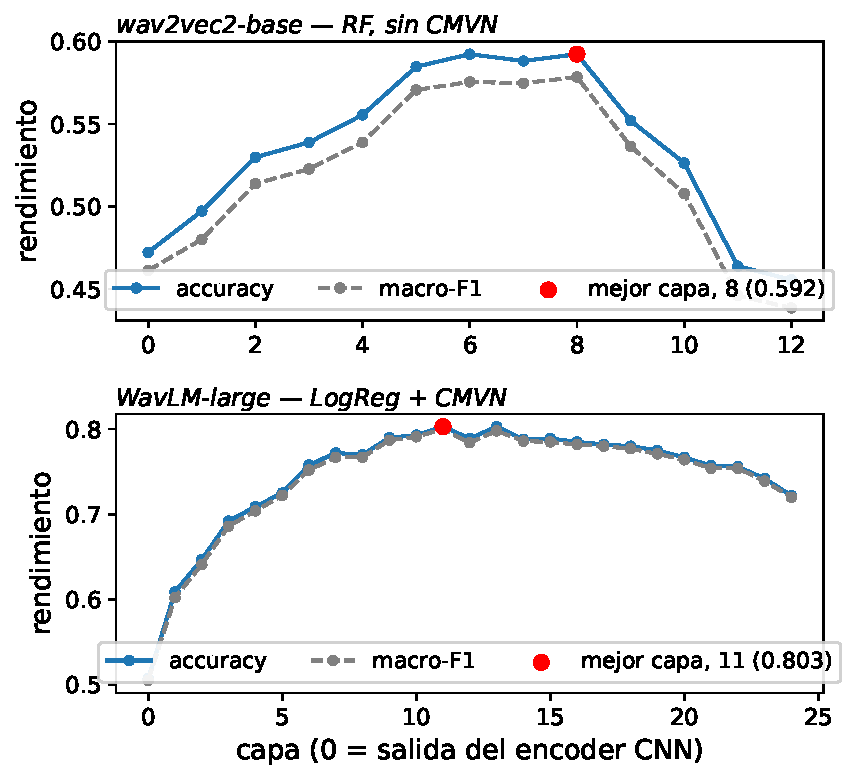
\includegraphics[width=\columnwidth]{layer_sweep}
\caption{Rendimiento por capa. Arriba se muestra wav2vec2-base (evaluado con
RF, sin CMVN) y abajo WavLM-large (LogReg $+$ CMVN). En los dos casos las
capas intermedias superan a las finales.}
\label{fig:sweep}
\end{figure}

\subsection{El efecto de normalizar por hablante}

La Tabla~\ref{tab:cmvn} aísla las dos mejoras de representación. CMVN por
hablante es la mejora individual más grande de todo el trabajo, con $+7$
puntos de accuracy sin tocar el modelo ($0{,}732 \rightarrow 0{,}803$). Eso
confirma que buena parte del error venía del confound de identidad. La
concatenación multi-capa suma unos 2 puntos más y eGeMAPS apenas medio
punto, señal de que la información experta ya está casi toda contenida en
los embeddings.

\begin{table}[t]
\caption{Efecto de CMVN y multi-capa (LogReg $C{=}0{,}01$, wav2vec2-base).}
\label{tab:cmvn}
\centering
\begin{tabular}{lcc}
\toprule
Representación & Accuracy & Macro-F1 \\
\midrule
capa 8 & 0,732 & 0,727 \\
capa 8 $+$ CMVN & 0,803 & 0,797 \\
top-3 capas & 0,736 & 0,731 \\
top-3 $+$ CMVN & 0,822 & 0,815 \\
top-3 $+$ eGeMAPS $+$ CMVN & \textbf{0,827} & \textbf{0,821} \\
\bottomrule
\end{tabular}
\end{table}

\subsection{Las redes neuronales no ganan}

Acá vino la primera sorpresa. Sobre la misma representación, el MLP quedó
por debajo del modelo lineal ($0{,}796$ contra $0{,}827$) y el CRNN sobre
secuencias frame-level, aun con acceso a la dinámica temporal completa,
quedó más abajo todavía ($0{,}763$). Con 1440 ejemplos la capacidad extra se
convierte en varianza, y los dos modelos sobreajustan sus folds a pesar del
dropout, el weight decay, el early stopping y los pesos de clase. El
resultado más caro confirmó el patrón. El fine-tuning end-to-end de
WavLM-large con aumentación llegó a $0{,}788$ en promedio (4 folds), lejos
del enfoque de features congeladas y con un costo computacional dos órdenes
de magnitud mayor. Con pocos datos, tocar los 317M de parámetros es peor que
dejarlos quietos.

\subsection{Optimización del sistema final}

La Tabla~\ref{tab:adv} resume el camino desde el mejor modelo individual
hasta el ensemble. Pasar a WavLM-large aporta $+3{,}7$ puntos sobre
wav2vec2-base y combinar representaciones suma $+0{,}9$. La aumentación de
pseudo-hablantes beneficia sobre todo al MLP ($0{,}847 \rightarrow 0{,}876$),
consistente con que las redes son las que más sufren la escasez de
hablantes. El ensemble de tres backbones llega a $0{,}882$, y con el MLP
aumentado más la ponderación final alcanza $\mathbf{0{,}890}$ / $0{,}888$ de
macro-F1. La Figura~\ref{fig:journey} resume el recorrido completo desde el
baseline. La Figura~\ref{fig:conf} muestra la matriz de confusión del
sistema final. Los errores que quedan se concentran en pares de activación
parecida, tristeza--calma (baja activación) y felicidad--sorpresa (alta).

\begin{figure}[t]
\centering
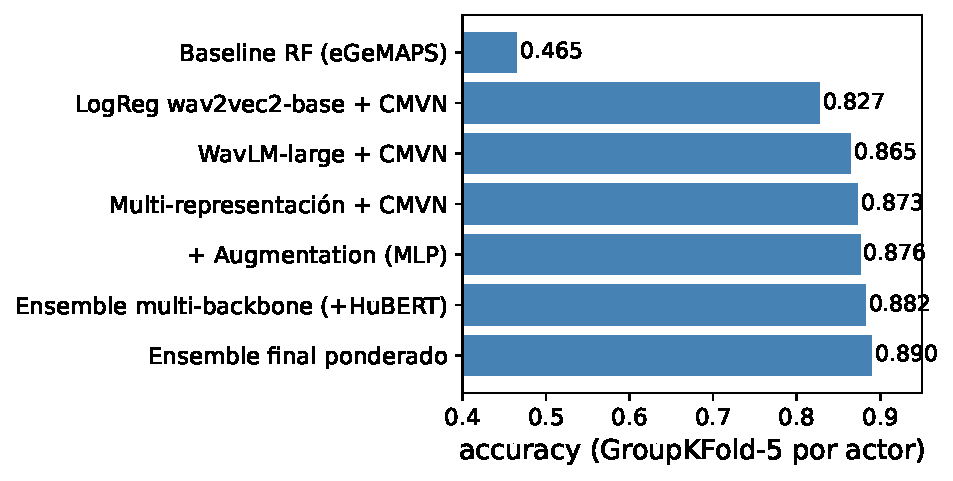
\includegraphics[width=\columnwidth]{journey}
\caption{Recorrido de optimización, del baseline al ensemble final.}
\label{fig:journey}
\end{figure}

\begin{table}[t]
\caption{Optimización avanzada y ensemble (speech, GroupKFold-5).
``base'' abrevia wav2vec2-base.}
\label{tab:adv}
\centering
\begin{tabular}{lcc}
\toprule
Sistema & Accuracy & Macro-F1 \\
\midrule
WavLM-large top-3 $+$ CMVN (LogReg) & 0,864 & 0,863 \\
WavLM $+$ base $+$ eGeMAPS $+$ CMVN & 0,873 & 0,871 \\
MLP (WavLM$+$base) $+$ aumentación & 0,876 & --- \\
Ensemble 3 backbones & 0,882 & 0,880 \\
Ensemble $+$ MLP aum. & 0,888 & 0,886 \\
Ensemble final ponderado (2-2-1-1) & \textbf{0,890} & \textbf{0,888} \\
\midrule
Fine-tuning WavLM-large $+$ aum. & 0,788 & 0,782 \\
\bottomrule
\end{tabular}
\end{table}

\begin{figure}[t]
\centering
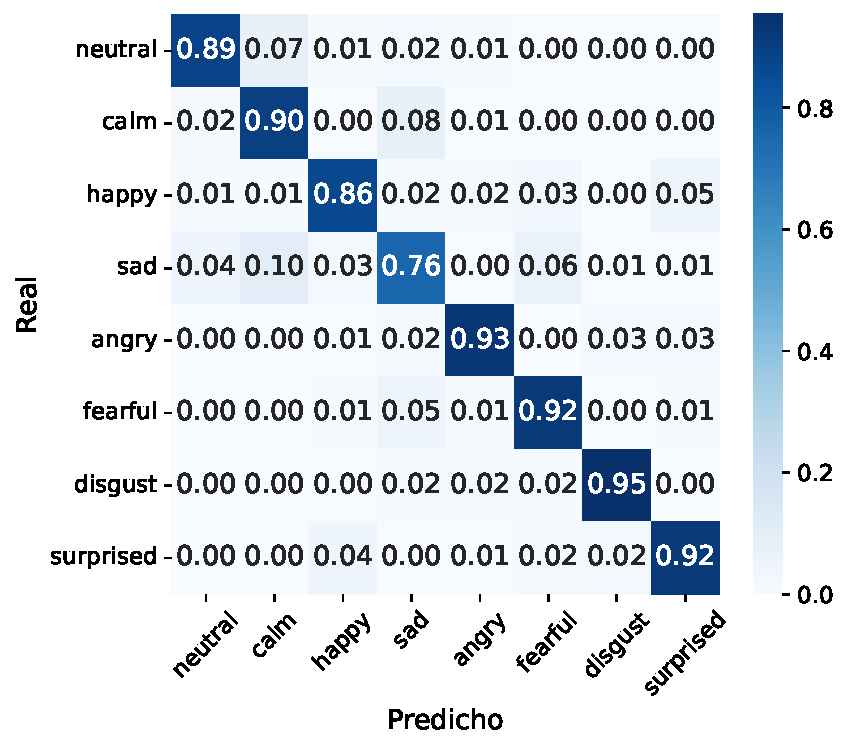
\includegraphics[width=\columnwidth]{ensemble_confusion}
\caption{Matriz de confusión (recall por clase) del ensemble final sobre
RAVDESS speech, predicciones out-of-fold.}
\label{fig:conf}
\end{figure}

\subsection{Diversidad sobre fuerza individual}

Un experimento posterior ilustra por qué funciona el ensemble, y es el
hallazgo que más nos gustó del trabajo. El MLP usa como entrada
WavLM$+$base. Al enriquecerlo con HuBERT su rendimiento individual mejoró
($0{,}874 \rightarrow 0{,}883$, su mejor valor aislado), pero el ensemble
\emph{empeoró} ($0{,}890 \rightarrow 0{,}887$). ¿Por qué? El MLP se volvió
más parecido a los votantes lineales, que ya usan HuBERT, y al promediar
aportó menos información nueva. En un ensemble importan más los errores no
correlacionados que la fuerza de cada miembro. El votante más débil pero
distinto complementa mejor que el más fuerte pero redundante.

En cuanto al sobreajuste, la validación speaker-disjoint elimina la vía
principal (memorizar voces), y la regularización fuerte, el early stopping y
la aumentación controlan la capacidad. Igual somos conscientes de un riesgo
más fino. Hicimos decenas de comparaciones contra el mismo protocolo de
validación cruzada, y elegir el mejor sistema con esas mismas métricas puede
sobreajustar la selección. Por eso importa la evaluación cross-corpus que
sigue, que es el único número del trabajo que el proceso de desarrollo no
pudo contaminar.

\subsection{Generalización cross-corpus (EMODB)}

La Tabla~\ref{tab:emodb} muestra qué pasa al aplicar el sistema final, sin
reentrenar, a un corpus en alemán. Sin ninguna adaptación el accuracy cae de
$0{,}890$ a $0{,}570$. Es una caída grande, pero queda muy por encima del
azar ($1/6 \approx 0{,}167$), señal de que los embeddings SSL capturan algo
de la emoción paralingüística que no es exclusivo del inglés. Aplicar CMVN
con las estadísticas de los hablantes de EMODB recupera casi 20 puntos
($0{,}767$), la mitad del camino de vuelta al rendimiento in-domain y con la
intervención más barata disponible. La Figura~\ref{fig:emodb} muestra que el
error dominante que queda es enojo clasificado como felicidad (36 de 127
casos). Tiene sentido acústico, porque las dos comparten activación alta
(energía y F0 elevados) y se distinguen por la valencia, que es la dimensión
más difícil de SER.

\begin{table}[t]
\caption{Cambio de dominio de RAVDESS a EMODB (454 audios, 6 clases).}
\label{tab:emodb}
\centering
\begin{tabular}{lcc}
\toprule
Variante & Accuracy & Macro-F1 \\
\midrule
Sin CMVN & 0,570 & 0,578 \\
Con CMVN por hablante & \textbf{0,767} & \textbf{0,787} \\
\bottomrule
\end{tabular}
\end{table}

\begin{figure}[t]
\centering
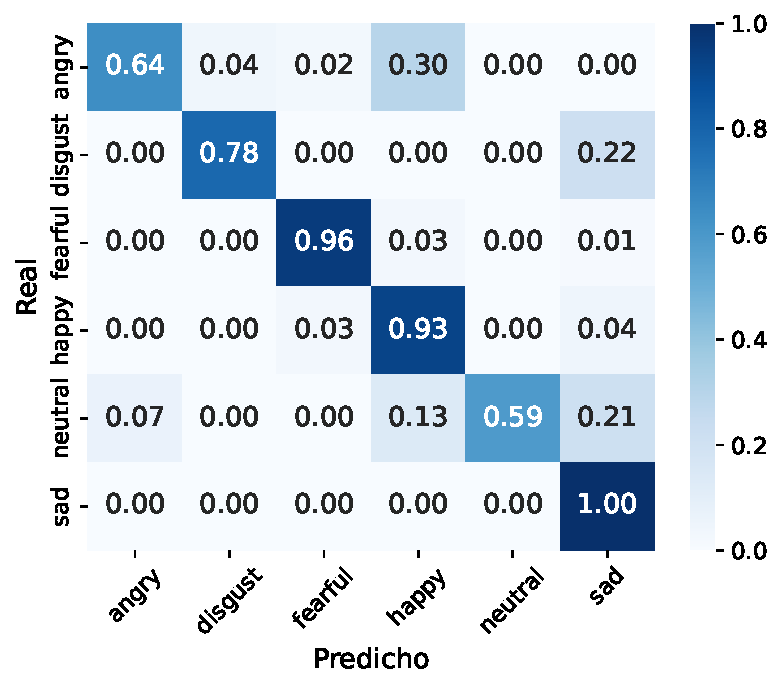
\includegraphics[width=0.92\columnwidth]{emodb_confusion}
\caption{Matriz de confusión (recall por clase) sobre EMODB con CMVN. El
error dominante es enojo $\rightarrow$ felicidad, pares de alta activación.}
\label{fig:emodb}
\end{figure}

\section{Conclusión y trabajo futuro}

Construimos un sistema de SER que mejora de $0{,}465$ a $0{,}890$ de
accuracy speaker-disjoint sobre RAVDESS. Las lecciones principales no son
las que esperábamos al arrancar. Primero, la ganancia dominante no vino de
modelos más grandes sino de controlar el confound de hablante (CMVN, $+7$
puntos). Segundo, con $\sim$1400 ejemplos los modelos lineales regularizados
le ganan a MLP, CRNN y fine-tuning end-to-end, y las redes solo aportan como
votante diverso de un ensemble. Tercero, en el ensemble la diversidad de
errores vale más que el rendimiento individual de cada miembro. La
evaluación cross-corpus sobre EMODB ($0{,}767$ sin reentrenar) sugiere que
el sistema captura emoción genuina y que normalizar por hablante es también
la herramienta clave frente al cambio de dominio.

Con más tiempo exploraríamos fine-tuning con corpus multilingües más grandes
(donde el enfoque end-to-end debería revertir su desventaja), calibración y
adaptación ligera al dominio destino (con unos pocos audios por hablante
alcanza para estimar CMVN, como mostró EMODB) y la dimensión de valencia,
que concentra los errores restantes.

\bibliographystyle{IEEEtran}
\begin{thebibliography}{9}

\bibitem{ravdess}
S.~R. Livingstone y F.~A. Russo, ``The Ryerson Audio-Visual Database of
Emotional Speech and Song (RAVDESS),'' \emph{PLoS ONE}, vol.~13, no.~5,
e0196391, 2018.

\bibitem{egemaps}
F.~Eyben \emph{et~al.}, ``The Geneva Minimalistic Acoustic Parameter Set
(GeMAPS) for voice research and affective computing,'' \emph{IEEE Trans.
Affective Computing}, vol.~7, no.~2, pp. 190--202, 2016.

\bibitem{opensmile}
F.~Eyben, M.~Wöllmer y B.~Schuller, ``openSMILE: the Munich versatile and
fast open-source audio feature extractor,'' en \emph{Proc. ACM Multimedia},
2010, pp. 1459--1462.

\bibitem{wav2vec2}
A.~Baevski, H.~Zhou, A.~Mohamed y M.~Auli, ``wav2vec 2.0: A framework for
self-supervised learning of speech representations,'' en \emph{Proc.
NeurIPS}, 2020.

\bibitem{wavlm}
S.~Chen \emph{et~al.}, ``WavLM: Large-scale self-supervised pre-training for
full stack speech processing,'' \emph{IEEE J. Sel. Topics Signal Process.},
vol.~16, no.~6, pp. 1505--1518, 2022.

\bibitem{hubert}
W.-N. Hsu \emph{et~al.}, ``HuBERT: Self-supervised speech representation
learning by masked prediction of hidden units,'' \emph{IEEE/ACM Trans. Audio,
Speech, Lang. Process.}, vol.~29, pp. 3451--3460, 2021.

\bibitem{pepino}
L.~Pepino, P.~Riera y L.~Ferrer, ``Emotion recognition from speech using
wav2vec 2.0 embeddings,'' en \emph{Proc. Interspeech}, 2021, pp. 3400--3404.

\bibitem{dogdu}
C.~Doğdu, T.~Kessler, D.~Schneider, M.~Shadaydeh y S.~R. Schweinberger, ``A
comparison of machine learning algorithms and feature sets for automatic
vocal emotion recognition in speech,'' \emph{Sensors}, vol.~22, no.~19,
7561, 2022.

\bibitem{emodb}
F.~Burkhardt, A.~Paeschke, M.~Rolfes, W.~Sendlmeier y B.~Weiss, ``A database
of German emotional speech,'' en \emph{Proc. Interspeech}, 2005, pp.
1517--1520.

\bibitem{sklearn}
F.~Pedregosa \emph{et~al.}, ``Scikit-learn: Machine learning in Python,''
\emph{J. Mach. Learn. Res.}, vol.~12, pp. 2825--2830, 2011. Se utilizaron
además PyTorch y HuggingFace Transformers.

\end{thebibliography}

\end{document}
